\documentclass[11pt,a4paper,titlepage,twocolumn]{ctexart}
\usepackage{mhchem,extarrows}
\usepackage{amsmath}
\usepackage{amsfonts}
\usepackage{amssymb}
\usepackage{graphicx}
\usepackage{hyperref}
\usepackage[left=2.54cm, right=2.54cm, top=3.18cm, bottom=3.18cm]{geometry}
\title{\textbf{{\huge 关于“测定空气中氧气的含量”实验的创新}}}
\author{青岛第二十六中学\quad 二〇一五级一班\\王愉扬}
\date{\today}
\begin{document}
	\maketitle
	\section{实验背景}
	
	在九年级上学期化学课本第7-1节中,介绍了测定空气中氧气的含量的方法,具体实验步骤如下:
	
\begin{center}
	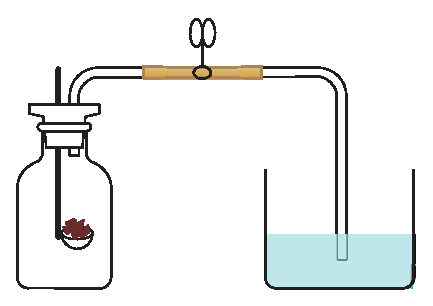
\includegraphics[width=0.8\linewidth]{fig/1}
\end{center}
	
	\begin{enumerate}
		\item 如图组装仪器,检查装置气密性.
		\item 在燃烧匙中装入过量红磷,置于酒精灯火焰上点燃后迅速放入集气瓶,塞紧瓶塞.
		\item 待燃烧完毕后容器恢复室温,打开止水夹,发现有一些水进入集气瓶内,且体积约占集气瓶体积的$\frac{1}{5}$.
		\item[·] 反应的化学方程式为:
		\[ \ce{4P + 5O2 \xlongequal{\mbox{\tiny 点燃}} 2P2O5}.\]
	\end{enumerate}

	由此,我可以得出\textbf{``空气中氧气体积约占$\mathbf{\frac{1}{5}}$''}这一结论.但是经过理论分析和课堂实际操作,发现这一方法的缺点主要有二:
	
	\begin{itemize}
		\item 红磷的着火点过高,导致在瓶外点燃的时间过长,浪费时间.
		\item 在瓶外点燃可能会导致气体逸散,导致实验不准确,结果有误差.
	\end{itemize}
	
	\section{实验改进}
	\subsection{改进点燃不便和气体可能逸散的问题}
	\begin{itemize}
		\item 针对第一个问题,我可以把红磷更换成白磷,经过查阅资料,我发现\textit{白磷的着火点约在40℃左右},便于被点燃,方程式如下:\[\ce{P4 + 5O2 \xlongequal{\mbox{\tiny 点燃}} 2P2O5}.\]
		\item 针对第二个问题,我可以把容器密闭,用凸透镜或聚能激光笔产生的集中热量来点燃固体,示意图如下:\\
		\begin{center}
			
\includegraphics[width=0.4\linewidth]{fig/2}
		\end{center}
		
	\end{itemize}
	
	我可以结合上述两种方案,设计出如下图所示的仪器:
	
	\begin{center}
		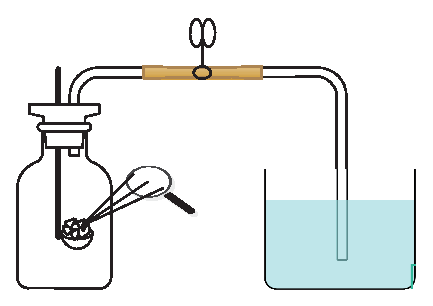
\includegraphics[width=0.8\linewidth]{fig/3}
	\end{center}
	

	经过测试,我又发现这套装置还是有如下缺点:
	
	\begin{itemize}
		\item 点燃还是不够方便,若没有凸透镜或激光笔,还是要用酒精灯点燃.
		\item 水在集气瓶中,只能靠目测体积——刻度不够直观,不利于理解该结论.
	\end{itemize}
	
	\subsection{改进点燃不方便和体积不直观的问题}
	
	\begin{itemize}
		\item 针对第一个问题,我上网查资料得知,\textit{白磷的着火点约为40℃左右},所以我可以直接把容器泡在开水中,这时,瓶内空气温度高于着火点,白磷就会自燃.
		\item 针对第二个问题,可以把水槽换成注射器,这样注射器减少的刻度就是消耗掉氧气的体积;再把集气瓶换成口径更细的试管,可以更加清晰地显示消耗氧气体积与总体积之比,示意图如下:\\
		\begin{center}
			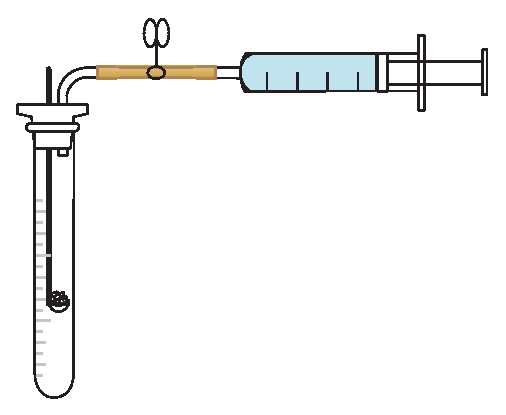
\includegraphics[width=0.8\linewidth]{fig/4}
		\end{center}
	\end{itemize}
		
	组合上述方案,又可以设计出如下图所示的仪器:
		
	\begin{center}
		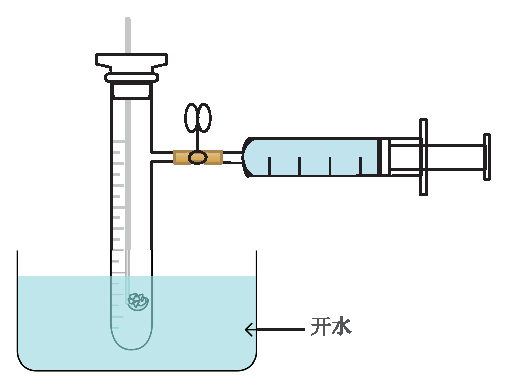
\includegraphics[width=0.8\linewidth]{fig/5}
	\end{center}
		
	经过试验,该套装置已能能较方便地点燃白磷,较好地反应体积的关系.但经过试验,仍发现了以下几个问题:
	
	\begin{itemize}
		\item 在试管中实验不太方便,特别是把燃烧匙伸入试管时容易撒漏.
		\item 注射器体积过小,装液量不够,不到集气瓶体积的$\frac{1}{5}$.
		\item 反应时放热,瓶内气压陡增,瓶塞容易弹开,需要在实验时用手按住. 
	\end{itemize}
	
	经过尝试,我决定把试管恢复到集气瓶,在瓶塞上添加压强平衡装置,并且把装有水的注射器换成量筒.
	
	经验表明,反应后产生的五氧化二磷( \ce{P2O5})有毒,且剩余的白磷也属于有毒易燃危险品,这在课堂应用中是不能实施的,下一步要解决的问题是处理反应残余物.
	
	\subsection{改进生成物不环保的问题}
	
	经过网上查阅资料,我发现, \ce{P2O5}可以通过与水反应来消耗掉,反应的方程式为:
	\[ \ce{P2O5 + 3H2O = 2H2PO4}.\]
	
	白磷可以与硫酸铜和水反应后生成无害物质,方程式为:
	{\footnotesize \[ \ce{P4 + 10CuSO4 + 16H2O = 10Cu + 4H3PO4 + 10H2SO4},\]}
	在水充足的情况下为:{\scriptsize \[ \ce{11P4 + 60CuSO4 + 96H2O = 20Cu3P + 24H3PO4 + 60H2SO4.}\]}
	
	在反应后的生成物中,\ce{H2PO4}、 \ce{H3PO4}、 \ce{Cu3P}均无毒无害,不会污染环境.
	
	在前一套装置中,水槽中的热水不能很好地靠近白磷,使引燃不够快,我想到可以把 \ce{CuSO4}加热,用瓶内的热 \ce{CuSO4}来接近白磷,减小引燃白磷的时间.
	\section{改进结果}
	\subsection{实验器材}
	
	集气瓶、橡皮塞、注射器、止水夹、燃烧匙、导管若干
	
	\subsection{实验药品}
	
	加热至70℃左右的 \ce{CuSO4}溶液、白磷
	
	\subsection{实验装置}
	
	\begin{center}
		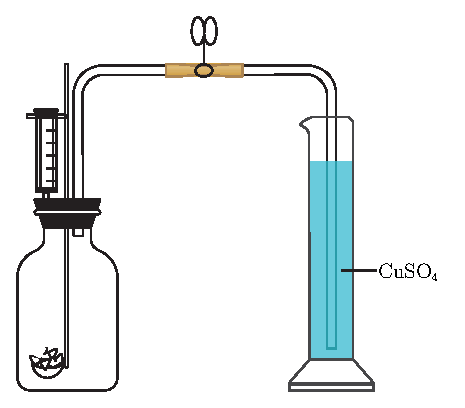
\includegraphics[width=0.6\linewidth]{fig/6}
	\end{center}
	
	\noindent\textbf{装置说明:} \indent\par
	\begin{description}
		\item[注射器] 在反应时平衡集气瓶内气压,防止反应时白磷放热导致瓶内气压过大使瓶塞弹开.
		\item[量筒] 显示被吸入集气瓶 \ce{CuSO4}的体积,刻度直观、准确.
		\item[\ce{CuSO4}] 反应前加热至高温后引燃白磷;反应后能够消耗有毒生成物.
	\end{description}
	
	\begin{enumerate}
		\item 如图,组装仪器.
		\item 检查装置气密性:打开止水夹,向上拉注射器活塞,使一部分高温 \ce{CuSO4}进入集气瓶,若注射器显示的体积等于量筒内液体减少的体积,则装置气密性良好.这时记录量筒中液面的位置.
		\item 关闭止水夹,把注射器活塞推到``0''刻度处,等待白磷被热 \ce{CuSO4}引燃.
		\item 待白磷燃烧后,可以看到气压平衡注射器的活塞向上移动.燃烧完毕后,把集气瓶放入冷水中,使集气瓶内温度尽快恢复到室温.待气压平衡注射器的活塞恢复到``0''刻度,用手摸瓶感到不热后,打开止水夹,可以观察到有一些 \ce{CuSO4}被吸入集气瓶,并且量筒中液面下降.
		\item 待液体不再进入集气瓶内,记录量筒内液面高度.用反应前的高度减去反应后液面高度,即可得到被白磷消耗的氧气体积.
		\item 得出结论后,向上拉动注射器活塞,使更多 \ce{CuSO4}进入集气瓶,没过燃烧匙.用力摇动集气瓶,使 \ce{P2O5}、水、 \ce{CuSO4}与白磷充分反应,完全消耗瓶内的残留物.
		\item 消耗尽残余物后,就可以打开瓶塞,拆卸、清洗装置了,不会出现空气污染的现象.
	\end{enumerate}
	
	\subsection{改进意义}
	
	\begin{enumerate}
		\item 改进了空气的逸散问题和燃烧物中白烟( \ce{P2O5})的污染.这样既能减少原来实验装置逸散空气的误差,也不污染环境,具有环保意识,防止空气污染.
		\item 注射器和量筒搭配巧妙.这一改进更加简化了读数环节,实验将清晰显示空气里 \ce{O2}的体积.同时,注射器和量筒都有精密的刻度,能直接读出精确的数值,提高了实验的准确性.
		\item 注射器能在白磷燃烧时缓冲集气瓶内气压的骤然增大,从而能防止冲塞现象的发生,起到了较好的缓冲作用
		\item 在引燃燃烧物\textit{(白磷)}方面设计巧妙.实验不仅方便操作,还环保,让实验现象更加容易观察.
		\item \textbf{总之,通过创新性地开展实验设计,在实验装置方面做了一些有益的改进,让实验更加精确,操作性更强;同时我在实验中也培养了实验探索、创新精神,发展了创新思维.}
	\end{enumerate}
	
\end{document}